% !TeX spellcheck = <none>

\documentclass[10pt,a4paper]{report}
\usepackage[a4paper, left=2cm, right=2cm, top=2cm, bottom=2cm]{geometry}
\usepackage[latin1]{inputenc}
\usepackage[arabic, english]{babel}
\usepackage{amsmath}
\usepackage{amsfonts}
\usepackage{amssymb}
\usepackage{graphicx}
\graphicspath{ {./images/} {../GeneratedPlots/} }
\usepackage{gensymb}
\usepackage{siunitx}
%\usepackage{matlab-prettifier}
\usepackage{float}
\usepackage[usenames,dvipsnames]{color} % color text
\usepackage{listings}
\usepackage{alphalph}
\usepackage[backend=bibtex]{biblatex} 
\addbibresource{References.bib}    
\usepackage[ddmmyyyy]{datetime}
\usepackage{caption}
\usepackage[toc,page]{appendix}

\usepackage{enumitem}
\usepackage{multicol}%try it out!

\usepackage{acronym}




\usepackage{etoolbox}
\makeatletter
\patchcmd{\chapter}{\if@openright\cleardoublepage\else\clearpage\fi}{}{}{}
\makeatother


\newcommand*\wildcard[2][6cm]{\vspace*{2cm}\parbox{#1}{\hrulefill\par#2}} %Wildcard for Signature line

\usepackage{lipsum} %random text




%Remove word "chapter" but leave numbering
\makeatletter
\renewcommand{\@makechapterhead}[1]{%
	\vspace*{50 pt}%
	{\setlength{\parindent}{0pt} \raggedright \normalfont
		\bfseries\Huge\thechapter.\ #1
		\par\nobreak\vspace{40 pt}}}
\makeatother

\usepackage[]{titlesec}
\titleformat{\chapter}[hang]{\huge\sffamily\bfseries}{}{0pt}{}[\hrule\vspace*{-23pt}] 

\usepackage{hyperref} %Load last as it can cause trouble with other packages. For Hyperlink https://de.wikibooks.org/wiki/LaTeX-W%C3%B6rterbuch:_hyperref

\newcommand{\HANSupervisor}{Wesselingh Ellen}
\newcommand{\CompanySupervisor}{Nguyen Trung}




\author{Karl Wallkum}


\begin{document}
	
		
	\begin{titlepage}
	\begin{flushright}
	\begin{minipage}{\linewidth}
		\begin{figure}[H]
			\begin{flushright}
			
\includegraphics[width=0.5\linewidth]{Images/HAN}
			%\caption{This is the first figure}
		\end{flushright}
		\hrule
		\end{figure}
		\begin{flushright}
			\large\textbf{ HAN Master Major Project}\\
			\vspace{20pt}
			\Huge\textbf{Major Project Plan
			\\
			\vspace{10pt}
			Using FANUC R-2000iC/210F\\
			(6-axis robot) for improved efficiency in FRC parts formation }
		\end{flushright}
		\vspace{35pt}
		\begin{figure}[H]
		\begin{flushleft}
		%	\includegraphics[width=0.25\linewidth]{Images/HAN_merk}
			%\caption{This is the second figure}
		\end{flushleft}	
		\end{figure}
		\begin{itemize}[leftmargin=4.5cm]
			\LARGE	
			\item[\textbf{Student Number:}] 617931		
			\item[\textbf{Name:}] Karl Wallkum 			
			\item[\textbf{Track:}] Master Control Systems Engineering
			\item[\textbf{Company:}]  HAN Smart Production Cell (IPKW)
			\item[\textbf{Supervisors:}]  \CompanySupervisor, (Company Supervisor)\\ \HANSupervisor, (HAN Supervisor)			
			\item[\textbf{Date:}] \today		 		
		\end{itemize}
	\end{minipage}
	\end{flushright}

	\begin{flushleft}
	\large \textbf{
		\vspace{40pt}
		\\HAN Smart Production Cell (IPKW)
	}
	%\vspace{10pt}
%	\\Arnhem, \hrulefill
%	\hspace*{0mm}\phantom{Arnhem, }Nguyen Trung

	\end{flushleft}
%\makebox[.5\linewidth][l]{Arnhem, }\dotsign\smallskip\\
%\hspace*{.5\linewidth}Nguyen Trung\\
%\hspace*{.5\linewidth}Title...

%\tabcolsep0pt
%\hfill\begin{tabular}{r{0.5\linewidth}@{}m{0.5\linewidth}@{}}
%	Approved:~ & Approved:~ \\\cmidrule{2-2} \cmidrule{4-4} 
%%	& Fats Domino, Ph.D.\\
%%	& Chair of the Department of Nutrition\\
%\end{tabular}

\begingroup
\centering
\wildcard{\CompanySupervisor}
\hspace{4cm}
\wildcard{\HANSupervisor}
\par
\endgroup


%\footnotetext[0]{template minor project report}
\end{titlepage}
	\begin{figure}[H]
	\centering
	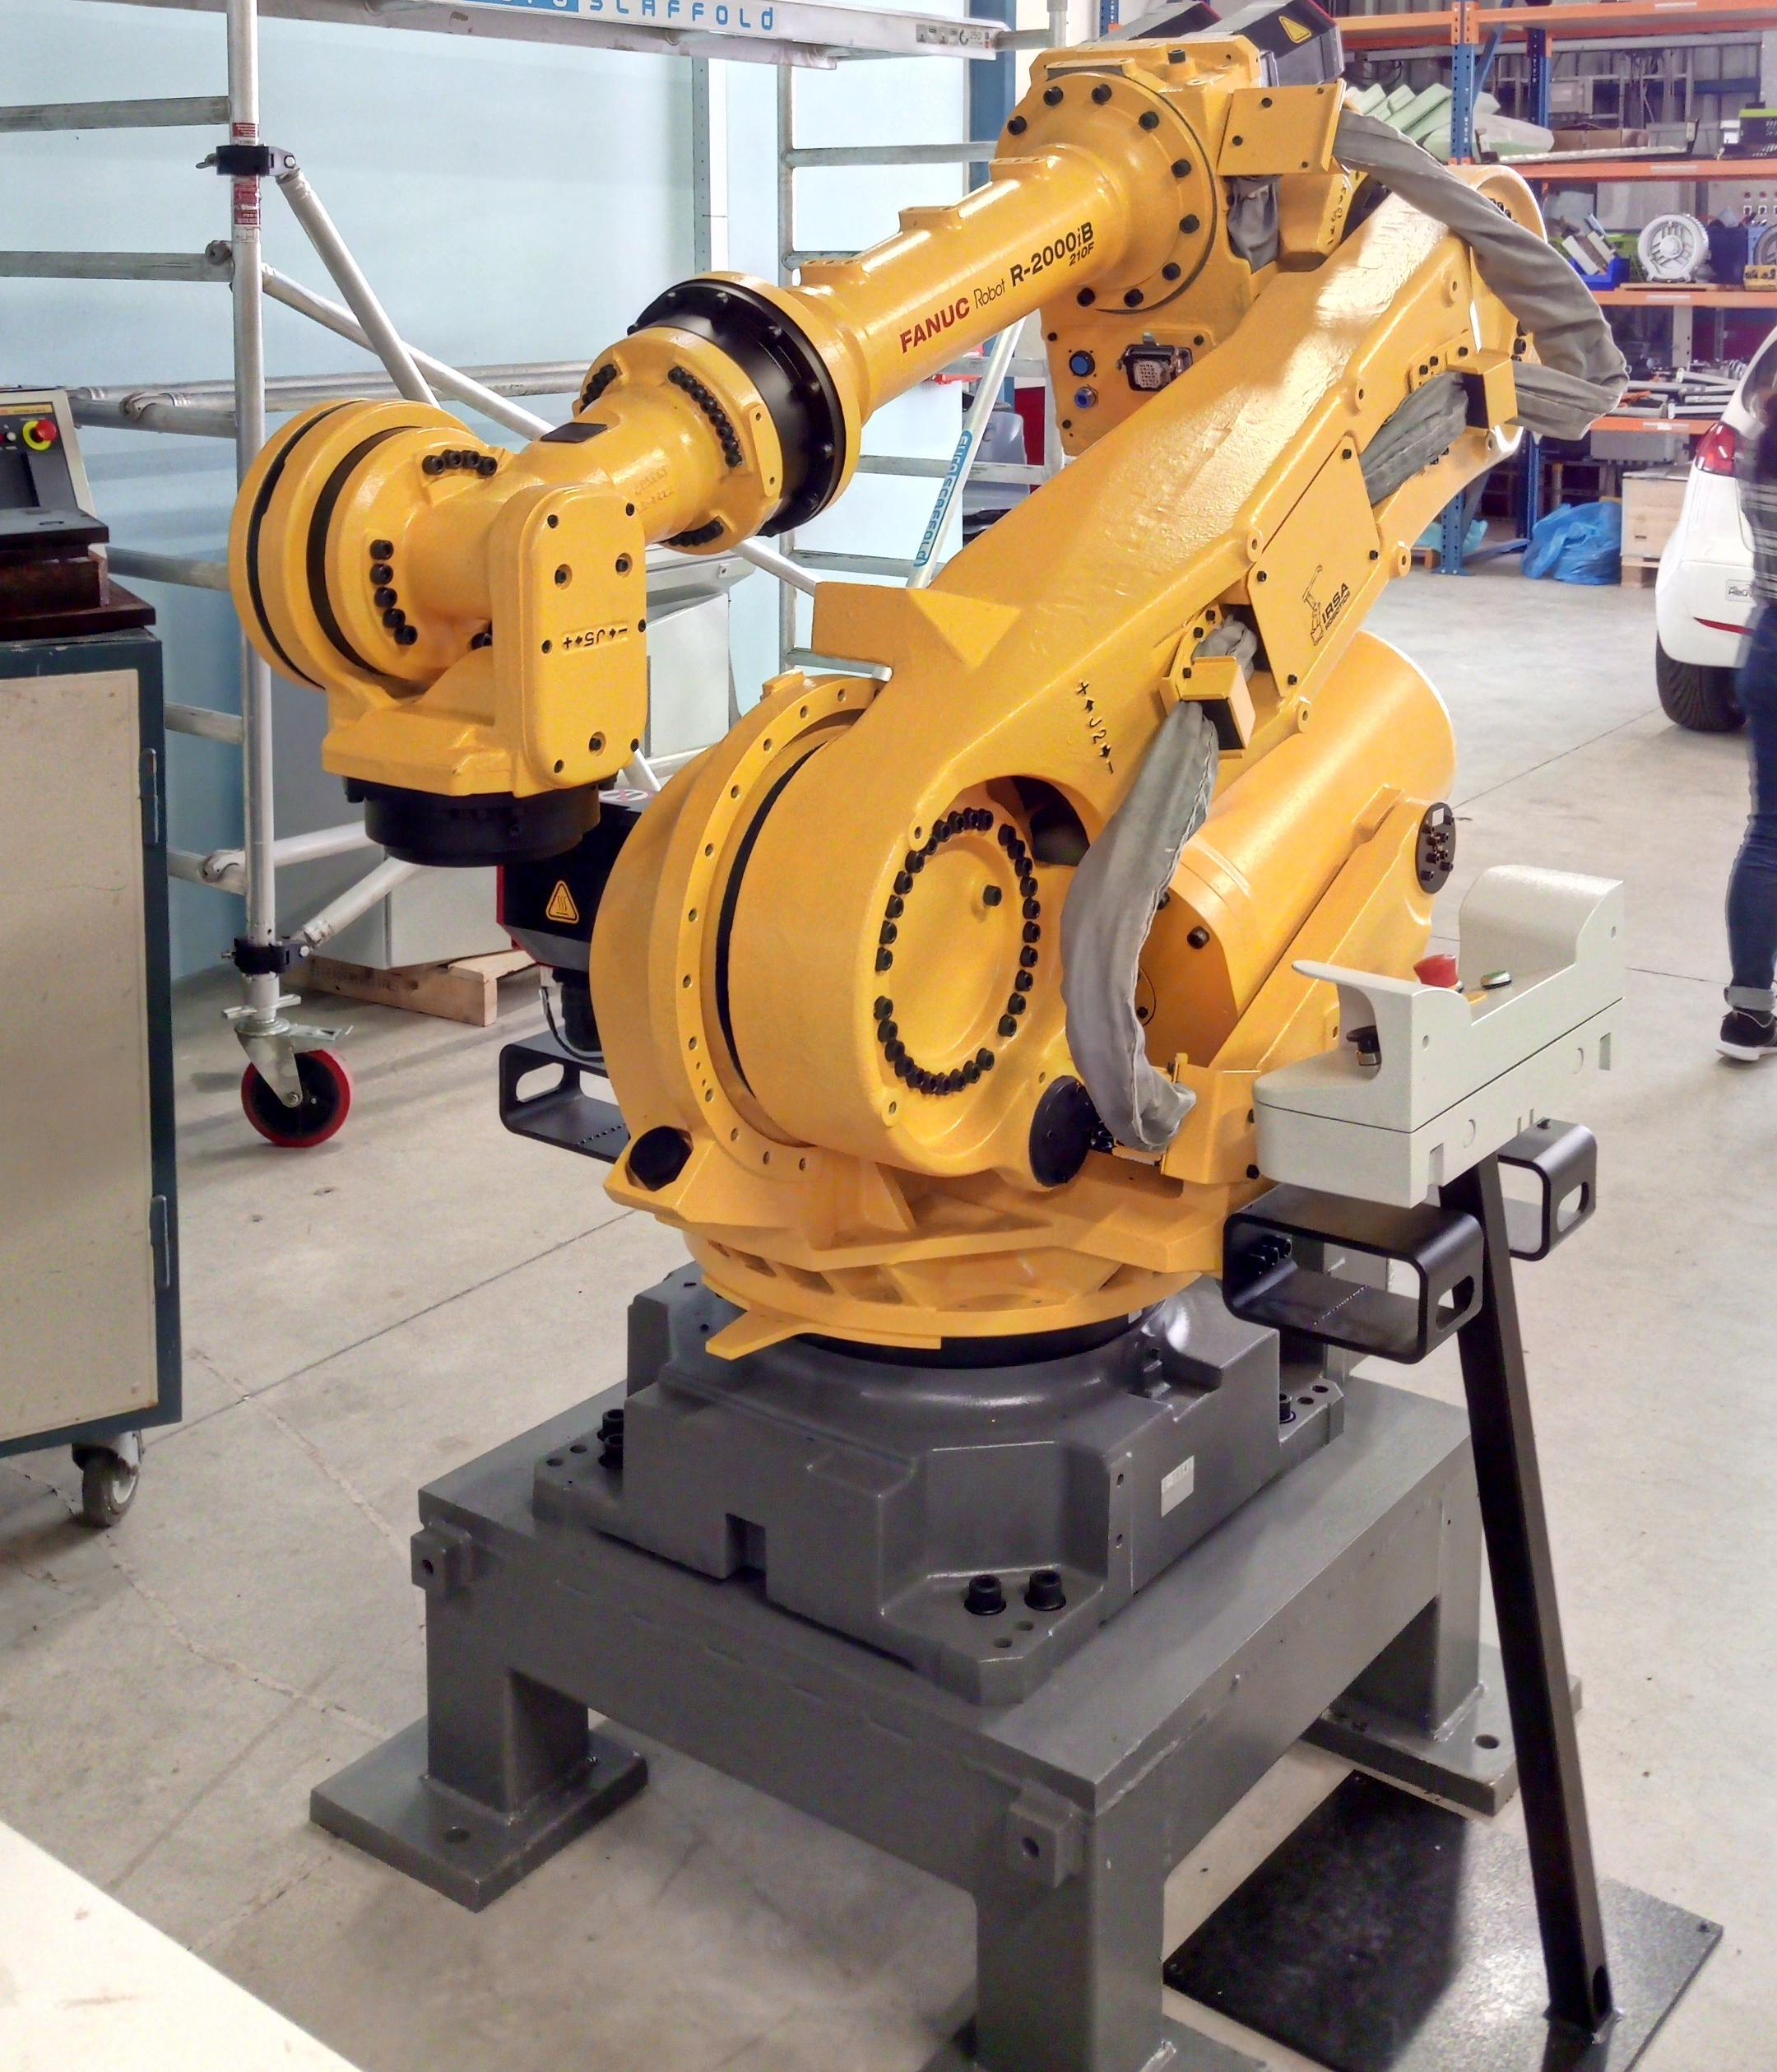
\includegraphics[
	width=1\linewidth,
	height=\paperheight,
	keepaspectratio,
	]{fanuc210_corner_cut}
	\caption{FANUC R-2000iC/210F 6-axis industrial robot arm}
	\label{fig:fanuc210}
\end{figure}
\pagestyle{empty}

	\cleardoublepage
		
	\tableofcontents
	
	\thispagestyle{empty}
	\clearpage
	\pagenumbering{arabic}
	
	%\section*{title}
The goal of this assignment is to ..\\
textextextext\\

\begin{table}[h]
	\centering
	\begin{tabular}{|l c l|}
		\hline
			&	&	\\
			&	&	\\
			&	&	\\
			&	&	\\
		\hline
	\end{tabular}
	\caption{caption}
	\label{Tab:table1}
\end{table}
%
textext as seen in Table \ref{Tab:table1} textextext.\\

\begin{figure}[H]
	\centering
	
\includegraphics[
	width=0.8\linewidth,
	height=\paperheight,
	keepaspectratio,
	]{testimage}
	\caption{Y vs X}
	\label{fig:image1}
\end{figure}

\newpage
	
	\chapter{Abstract}
%~150Words

This work aims to integrate a FANUC 210F 6 axis industrial robot arm  into an experimental production line. 
As this production line is set in a research environment, gaining a deeper understanding of all involved systems is desired.\\
\\
The dynamic behaviour of a physical system is best expressed with an analytical model.
In order to control a robot arm, a kinematic model needs to be created. With this model, a control algorithm can be derived.\\
\\
The objective of this thesis is to derive the complete inverse kinematic model of a 6 \ac{DOF} robotic arm analytically. For an exact numerical simulation of the device most steps are laid out theoretically and difficulties in the practical implementation are described.
Additionally for follow up projects this work also contains a quick start guide and a safety manual for the robot in this setting .
Finally to contribute to current research, twinning specifications will be defined.


%See: https://www.sfu.ca/~jcnesbit/HowToWriteAbstract.htm
%
%%What is an Abstract?
%
%The abstract is an important component of your thesis. Presented at the beginning of the thesis, it is likely the first substantive description of your work read by an external examiner. You should view it as an opportunity to set accurate expectations.
%The abstract is a summary of the whole thesis. It presents all the major elements of your work in a highly condensed form.
%An abstract often functions, together with the thesis title, as a stand-alone text. Abstracts appear, absent the full text of the thesis, in bibliographic indexes such as PsycInfo. They may also be presented in announcements of the thesis examination. Most readers who encounter your abstract in a bibliographic database or receive an email announcing your research presentation will never retrieve the full text or attend the presentation.
%An abstract is not merely an introduction in the sense of a preface, preamble, or advance organizer that prepares the reader for the thesis. In addition to that function, it must be capable of substituting for the whole thesis when there is insufficient time and space for the full text. 
%
%
%%Size and Structure
%
%Currently, the maximum sizes for abstracts submitted to Canada's National Archive are 150 words (Masters thesis) and 350 words (Doctoral dissertation)
%The structure of the abstract should mirror the structure of the whole thesis, and should represent all its major elements.
%%For example, if your thesis has five chapters (introduction, literature review, methodology, results, conclusion), there should be one or more sentences assigned to summarize each chapter. 
%
%
%%Clearly Specify Your Research Questions
%
%As in the thesis itself, your research questions are critical in ensuring that the abstract is coherent and logically structured. They form the skeleton to which other elements adhere.
%They should be presented near the beginning of the abstract.
%There is only room for one to three questions. If there are more than three major research questions in your thesis, you should consider restructuring them by reducing some to subsidiary status. 
%
%Don't Forget the Results
%
%The most common error in abstracts is failure to present results.
%The primary function of your thesis (and by extension your abstract) is not to tell readers what you did, it is to tell them what you discovered. Other information, such as the account of your research methods, is needed mainly to back the claims you make about your results.
%Approximately the last half of the abstract should be dedicated to summarizing and interpreting your results. 


%%Example and Tips: https://www.scribbr.de/aufbau-und-gliederung/abstract-schreiben/







	
	% !TeX spellcheck = <none>
%testtest
\chapter{Background}


	\chapter*{Acknowledgements}

I want to thank everyone who has helped me with this thesis work. It was a great learning experience for me.\\
\\
First of all, I would like to thank Peter Verschut, the project manager at SPC, who has made this project possible. By providing the SPC lab at MIC and letting me do experiments with the machines, I could get a lot of practical experience with the Fanuc210F and other machines. Also he connected me with experts in the field so I could make contacts for further work in the field of robotics. \\
\\
Dimitri Jeltsema gave me a good hint how to model and control the robot based on the content of his lectures. Besides that, Ellen Wesselingh and Trung Nguyen have given me great advice on the writing and modelling of the robot. Without your guidance this journey would have been a lot harder. Your critical questioning and pushing in the right direction have helped me a lot. Thank you for your patience and effort. \\
\\
Peter Corke has made the modelling and control of the robot arm a lot easier for me with the toolbox that he distributes for free. I hope, this toolbox will see many more iterations with additional functionalities and improvements.\\
\\
Aliya Patel, a fellow master student working on another type of robot was a great help in the practical part of the project. Also besides the work, I am happy to have you as a friend. I wish you success in your career and I hope you will get to work in your field of interest.\\
\\
Also Didier, Suzanne, Ivan and the other employees and students at SPC were always there, when I needed a helping hand. We were a great team.\\
\\
I would also like to thank Bram and his colleagues from Qing for the great collaboration.\\
\\
Special thanks goes to Karlijn who has kept me sane in times of isolation due to Covid-19. Thanks for the moral support!\\
\\
Finally, I would like to thank my Mother and her partner Gerhard for making this master studies possible for me.

	% !TeX spellcheck = <none>
%testtest
%\chapter{Summary}


	
	\chapter{Acronyms}
\begin{acronym}[Bash]
	\acro{HAN}{Hogeschool van Arnhem en Nijmegen}
	\acro{SPC}{Smart Production Cell}
	\acro{DOF}{degrees of freedom}
	\acro{FRC}{Fibre Reinforced Composites}
	\acro{DH}{Denavit-Hartenberg}
	\acro{IOT}{Internet Of Things}
	\acro{FHEM}{Freundliche Hausautomation und Energie-Messung \cite{FHEM}}
	\acro{NFC}{Near-field communication}
	\acro{IPKW}{Industrial Park Kleevse Waard}
	\acro{NFC}{Near Field Communication}
	\acro{ROS}{Robot Operating System}
	\acro{GUI}{Graphical User Interface}
	\acro{EOAT}{End Of Arm Tooling}
	\acro{PL}{Production Line}
	\acro{ETCS}{European Train Control System}
	\acro{DT}{Digital Twin}
	
\end{acronym}



	
	\input{Background/Context}
	\input{Background/IndustryRelevance}
	\input{Background/OriginOfProject}
	\input{Background/Fieldlab}
	
	\section{Problem Definition}

For \ac{FRP} part production, a robot arm can be used to load the press with raw material and unload the finished product. This allows for more flexibility in the production line than specialized low \ac{DOF} pick and place systems.
For this task, a Fanuc 210F was obtained by \ac{SPC}. The robot was delivered by IRSA Robotics. As the robot was not yet ready to carry out any task, setup and commissioning was necessary. 

%As the robot arm has many degrees of freedom, there are different strategies for a control cycle. 
%There are two contractionary main constraints that need to balanced:
%On one hand, the movement of materials has to be achieved as fast as possible to minimize the cool-down of the molten \ac{FRP}. 
%On the other hand, the accelerations and forces on it should be minimized while transferring, to make sure no material is lost in the transfer process which would lead to deformations on the final product.
%This makes it hard to find an ideal, fast control strategy to place the raw material into the press.
\medskip

\section{Objective}

This thesis describes the setup, modelling and control of a 6\ac{DOF} serial link industrial robot arm in a pick and place application for a production line. A combined kinematic and dynamic model of the Fanuc 210F is obtained. This model is then used to create a model-based control for the intended pick and place operation in the production line.


	
	\input{Objectives/Objectives}
	
	\input{Approach/Approach}
	
	\input{Outline/Outline}
	
	
	\input{ThesisWork/Introduction}
	
%	\input{ThesisWork/}
	
	\chapter{Literature survey}

In my project plan I stated that "I will demonstrate my master level by understanding and simulating the dynamics of a 6 axis Robot arm."\cite{ProjectPlan}
This should be done by creating a model of the robot arm. This model can then be used to create a controller.
To create the model of the robot arm, a literature review is necessary to lay out the best approach.\\
\\
Additionally to the modelling and control of the robot arm, digital twinning became a research topic within the project. A review of existing literature on digital twinning will be done as well.
\medskip

\section{Field of study}

To start the literature review, a set of first keywords was needed. Through an expert interview with my company supervisor Trung Nguyen \cite{Trung} , who had already supervised other thesis projects in the domain of robotics, a list of keywords to start with was found in a quick discussion. Not all of these keywords were immediately clear, so it was necessary to find definitions for these. With the help of scientific databases and search engines, sources for these definitions could be found.\\




	\begin{itemize} [leftmargin=3cm]
		\item [\textbf{6 axis robot}] serial 6 degree of freedom robots (\cite{6axisRobot} with HANQuest)
		\item [\textbf{industrial robot arm}]  some form of jointed structure  achieved by the linking of a number of rotary and/or linear motions or joints( \cite{IndustrialRobotArm} with Science Direct)
		\item [\textbf{inverse kinematics}]  mathematical process of recovering the movements of an object with kinematic equations to determine the joint parameters that provide a desired position for each of the robot's end effectors (\cite{InvKinDef} with Wikipedia)
		\item[{\parbox[t]{0.25\linewidth}{\textbf{Peter Corke \\ robotics toolbox}}}] \parbox[t]{1\linewidth}{Matlab toolbox for the study and simulation of classical arm-type robotics, for example such things as kinematics, dynamics, and  trajectory generation (\cite{CorkeRoboticsToolbox} with Google search)}
		\item [\textbf{motion planning}]  find a sequence of valid configurations that moves the robot from the source to destination (\cite{MotionPlanning} with Google search)
		\item [\textbf{robot dynamics}] relationship between the forces acting on a robot mechanism and the accelerations they produce (\cite{RobotDynamics}, with Scholarpedia)
		\item [\textbf{ROS}] Robot Operating System - framework for writing robot software. It is a collection of tools, libraries, and conventions that aim to simplify the task of creating complex and robust robot behaviour across a wide variety of robotic platforms. (\cite{ROS} with Google search )
		%manual linebreak in item label
%		\item[{\parbox[t]{0.2\linewidth}{force here \\ a linebreak}}] Some text right of the label 
\end{itemize} 
\medskip

As seen in "Implementation of Robot Systems" \cite{IndustrialRobotArm}, the FANUC 210F is an articulated robot arm, also called a jointed arm. It is a 6 axis robot that has six rotational joints, each mounted on
the previous joint. This type of robot has the ability to reach a point within the working envelope in more than one configuration or position. 
As there are multiple configurations possible to reach the same position, path planning would become an important topic. 
This means through inverse kinematics  the motion of the joints needs to be determined without considering the local forces that cause them to move.
The robotics toolbox by Peter Corke was seen as a good tool for simulating these kinematics in MATLAB. 
When attaching the dynamics to this model, further simulations could be made to simulate the dynamic bahaviour of the robot arm and create a controller. %power demand to move the joints with the desired speed. 
%As it became clear, that it would be difficult to determine the inertias, spring and damping forces on the robot within the given time, a pure kinematic analysis was seen sufficient.
ROS, while being an advanced tool for robot control would not fall in the scope of this thesis, as it would rather be a tool for later in the process of integrating the robot into the production line.\\
\medskip

\section{In depth literature}

As stated in the online manual of MathWorks, "Kinematics is the study of motion without considering the cause of the motion, such as forces and torques." \cite{MathWorksInverseKinematics}
Inverse Kinematics, also called backward kinematics is the logical opposite to forward kinematics also called direct kinematics (See figure \ref{fig:FwVsInvKin}). 


\begin{figure}[H]
	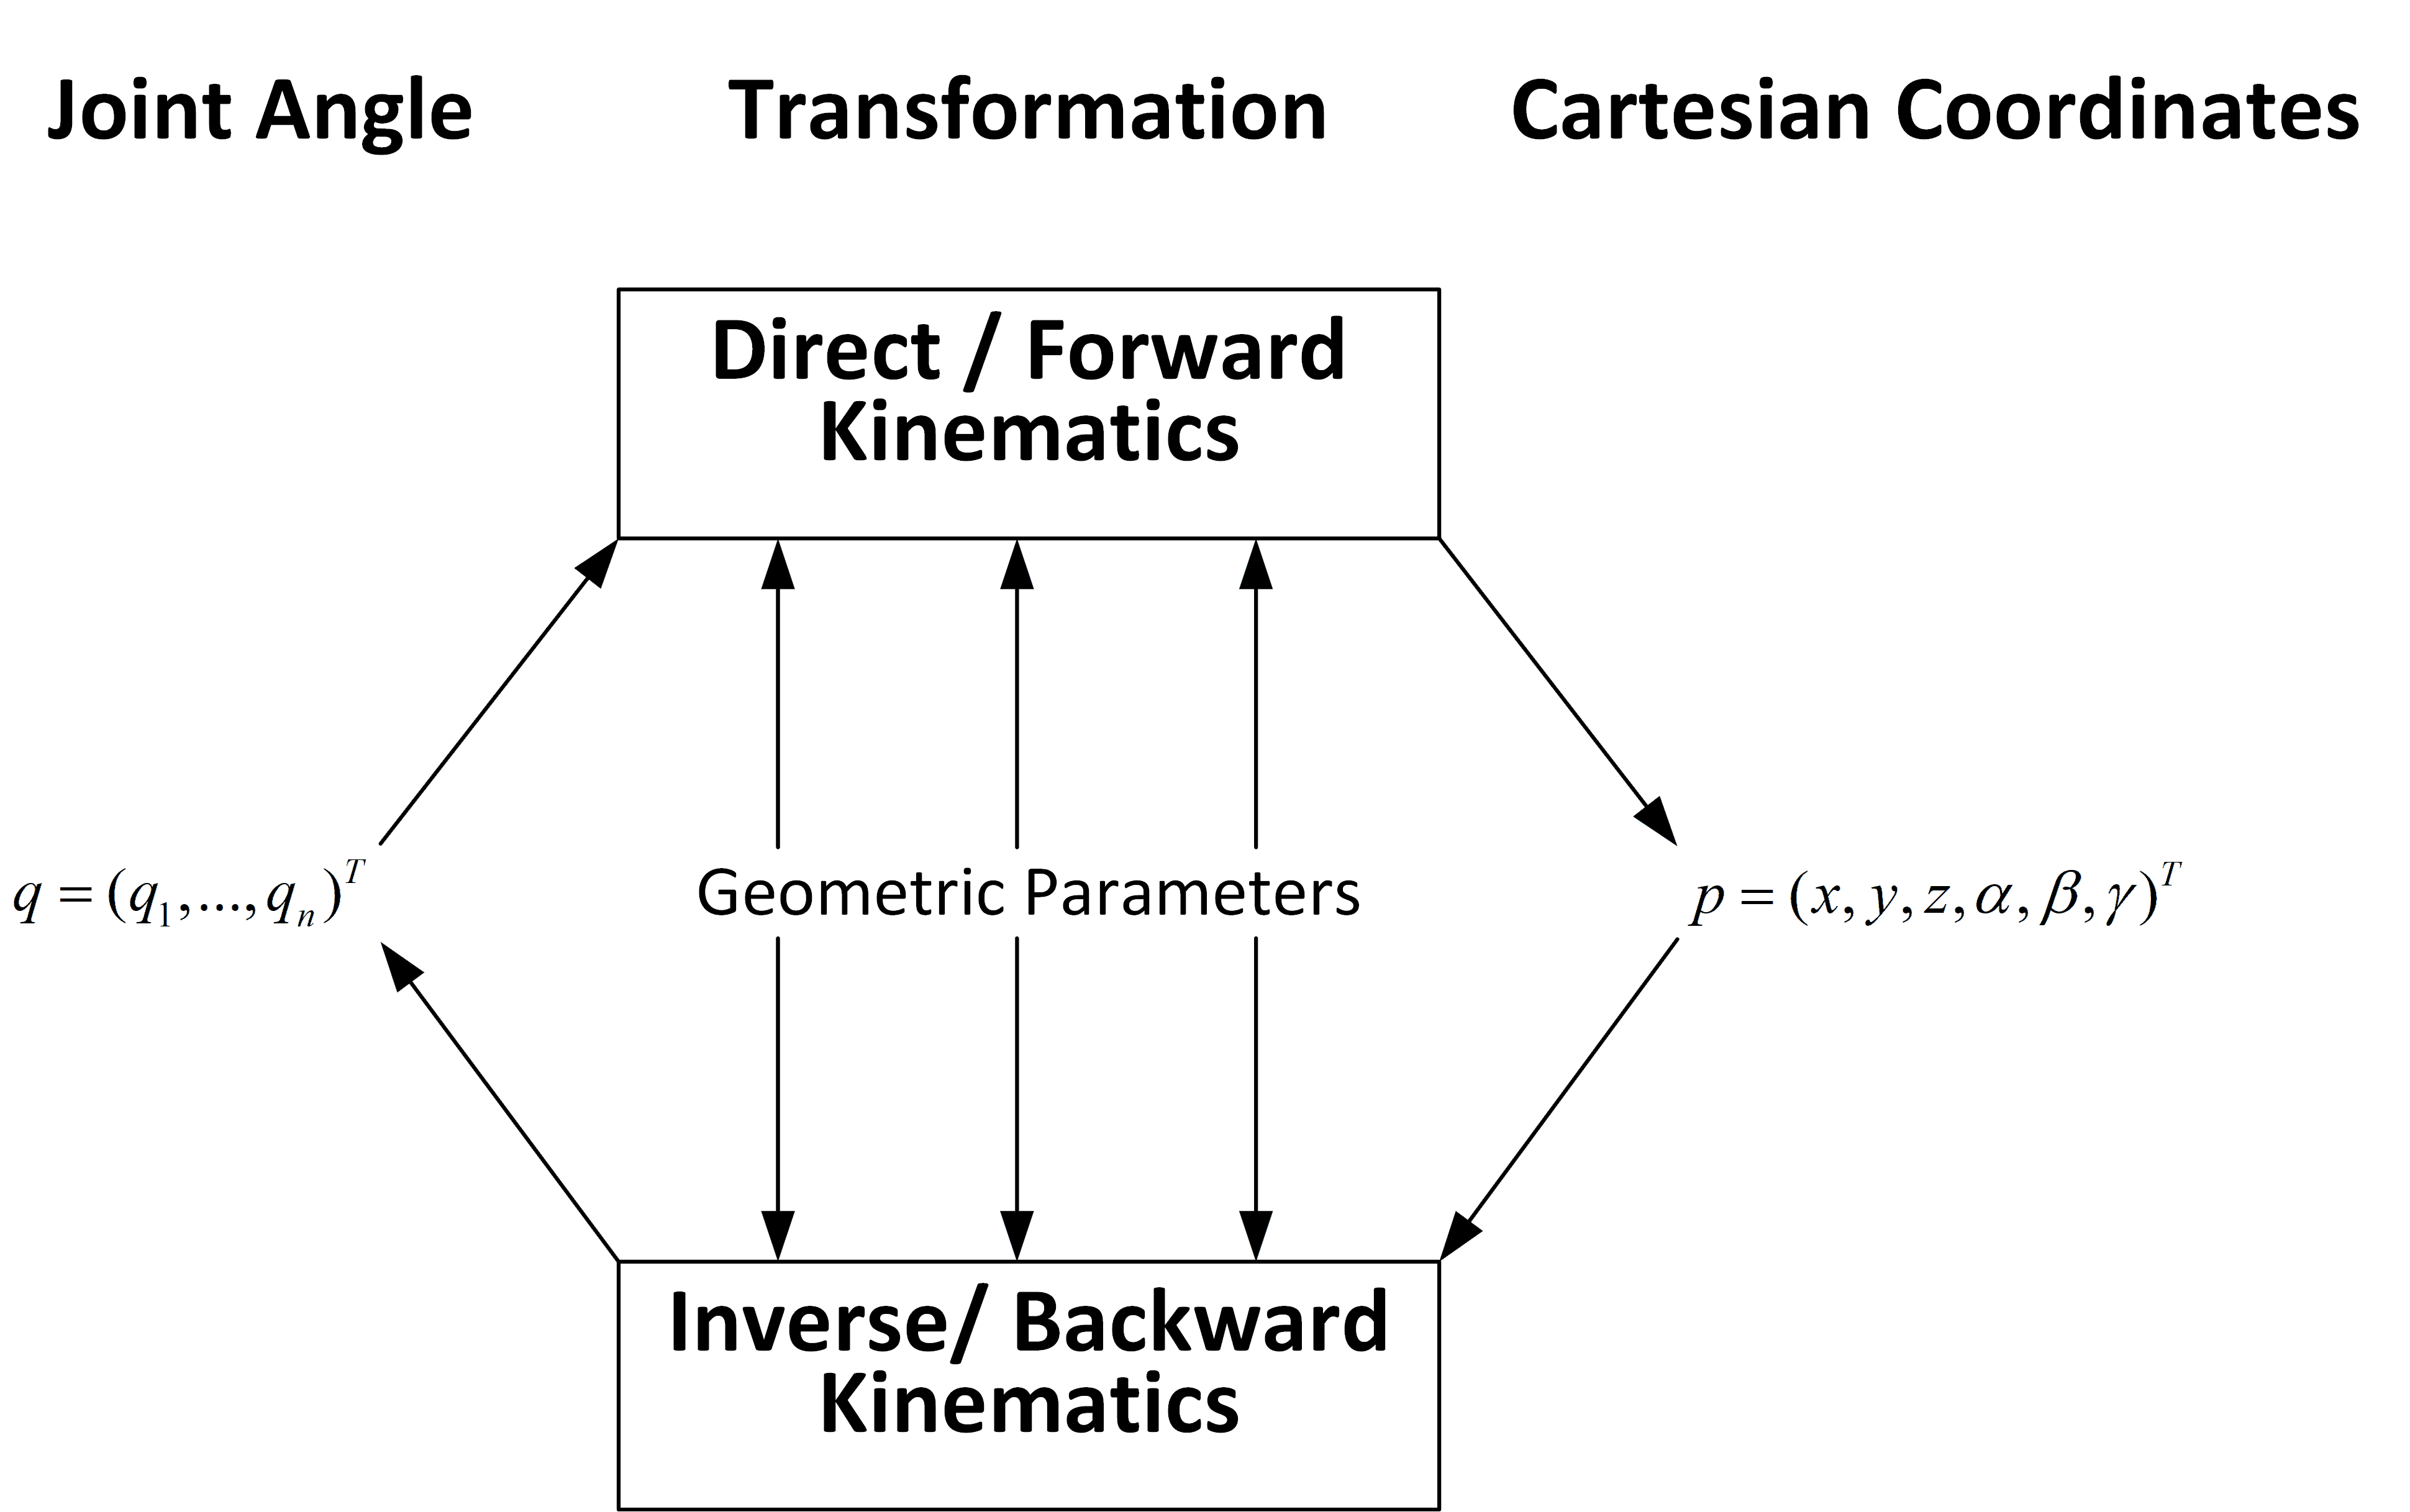
\includegraphics[
	width=0.95\linewidth,
	right,
	keepaspectratio,
	]{VisioDrawings/FWDvsINV_Kinematics_HighResTransp}
	\caption{Relation between inverse and forward kinematics translated from German Wikipedia site on inverse inematics \cite{forwardVsInverseKinematics}}
	\label{fig:FwVsInvKin}
\end{figure}

In the german wikipedia article on inverse kinematics \cite{inverseKinematikWiki}, the thesis "Verallgemeinerte inverse Kinematik für Anwendungen in der Robotersimulation und der virtuellen Realität" \cite{allgInvKin} is given as one of the main sources. 
This thesis work gives a good overview on the topic of inverse kinematics. 
As stated in this thesis work, the Denavit-Hartenberg notation is a robotic convention to map the local coordinate systems within a kinematic chain as found in robot arms.

As seen in "A Mathematical Introduction to Robotic Manipulation" \cite{MathIntroRobManip} (obtained through Semantic Scholar, search phrase: robotic convention), there are several other conventions besides the "Denavit-Hartenberg notation" used in the robotics research field like the the "product of exponentials formulation".
%Another overview on robotic conventions can be found in the Wikipedia article on robotic conventions \cite{RobConventionsWiki}. 
As most literature prefers a Denavit-Hartenberg fomulation of the kinematics (see \cite{MathIntroRobManip}), this convention will be chosen in this work as well.

Solutions for forward  kinematics are simple to obtain but solving inverse kinematics  has  been  one of  the  main  concerns  in  robot kinematics research. 
With more \ac{DOF}, solutions get more complex as non-linear equations with transcendental functions need to be solved. 
For this set of equations, no general algorithms are available.
Often algebraic, geometric and iterative methods for complex manipulators are used to find a solution to the inverse kinematic problem as stated by Tarun Pratap Singh et al. \cite{FwdInvAnalysRobManip}.

To find a suitable method for solving the inverse kinematic problem, a definition for the solution is needed:\\
\medskip
\\
\fbox{\parbox{\textwidth}{"A manipulator will be considered solvable if the joint variables can be determined by an algorithm that allows one to determine all sets of joint variables associated with a given position and orientation. [...] The algorithm should find all possible solutions" -Dr.-Ing. John Nassou\cite{invKinSeriallinkMani}}}
\bigskip

With this definition of solvability, all systems with revolute and prismatic joints with 6 \ac{DOF}  in a single series chain are solvable with the current available research. \cite{invKinSeriallinkMani}
As a quick search on HAN Quest with the search term "7 DOF inverse kinematics" suggests, there is currently onging research for the inverse kinematics problem in higher DOF manipulators with fuzzy logic as multiple articles following this approach can be found.\\
\\

As the goal is to find a suitable solution strategy for the inverse kinematic problem, it helps to map out the different types of methods.
Solution strategies can be split into two classes as stated by Dr.-Ing. John Nassou \cite{invKinSeriallinkMani}:\\
\medskip


%\parbox[t][3cm][t]{7cm}{\normalsize Closed-form solutions\\}
%\parbox[t][3cm][t]{7cm}{\normalsize Numerical solutions\\} 
%Text on two sides of the page:%https://tex.stackexchange.com/questions/107491/left-and-right-aligned-text-boxes
\fbox{\begin{minipage}[t]{0.6\textwidth}
	\textbf{{\large Closed-form solutions}}\\
	faster because analytical method\\
	will find all solutions\\
	Two approaches:\\
	\\
	\begin{minipage}[t]{0.4\textwidth}
		\textbf{{\large algebraic approach}}\\
	\end{minipage}
	\begin{minipage}[t]{0.4\textwidth}
	\begin{flushright}
	\textbf{{\large geometric approach}}\\
	\end{flushright}
\end{minipage}
\end{minipage}
\hfill
\begin{minipage}[t]{0.35\textwidth}
	\begin{flushright}
		\textbf{{\large Numerical solutions}}\\
		slower because of iterative nature\\
		not always find all solutions\\
	\end{flushright}
\end{minipage}}
\medskip

As numerical methods solve within an unknown number of operations, cannot always deliver  all solutions and depend on the users decision for accuracy, \cite{invKinSeriallinkMani} a closed-form solution will be preferred.

On HAN Quest, with the keywords "6DOF inverse kinematics" the article "Inverse Kinematics Solution and Optimization of 6DOF Handling Robot" \cite{invKinSolYanWu} can be found. This offers an  algebraic method to solve the inverse kinematic problem for 6 axis robots.
A similar approach is shown in "Forward and Inverse Kinematic Analysis of Robotic Manipulators" \cite{FwdInvAnalysRobManip}\\

As an alternative, a geometric modeling can be done as seen in "Workspace analysis and geometric modeling of 6 DOF Fanuc 200IC " \cite{geomModelingKamel}. 
A completely different approach is given in "A inverse kinematic solution of  a 6-DOF industrial robot using ANN" by using artificial neural networks \cite{invKinANNKSHITISH}.\\
%https://www.tu-chemnitz.de/informatik/KI/edu/robotik/ws2016/lecture-ik%201.pdf
%
%We will split all proposed manipulator solution strategies into two broad classes:Closed-form solutions and numerical solutions.Because of their iterative nature, numerical solutions generally are much slower than closed-form solutions and do not assure to really find all solutions.For most uses, we are not interested in the numerical approach to solve inverse kinematics.Here, we will restrict our attention to closed-form solutions.In this context, we search for solutions based on an analytic expression.
%Robots, for which a closed-form solution exists, are characterized either by having several intersecting joint axes or by having many twist angles αibe equal to0 or+/-90°.
%
With one of these methods, a solution can be found for the inverse kinematic problem.
This solution can then be verified with the robotics toolbox (Corke)

With this solution, a dynamic model of the robot can be created by attaching dynamics to the model as seen in "Control and Safety Mechanisms for a 3 DOF Manipulator with Human Interaction" \cite{KongWei} and "A mathematical introduction to Robotic Manipulation" \cite{MathIntroRobManip}. A complete example of a dynamic simulation of a 6 \ac{DOF} robot arm can be found in "Dynamic Multibody Simulation of a 6-DOF Robotic Arm" \cite{Dyn6DOFBinLi}

A controller for trajectory tracking can then be created with the model as seen in "Experimental Evaluation of Nonlinear Feedback and Feedforward Control Schemes for Manipulators" \cite{evalNonlinFeedForBackControl}

This controller could then be plugged into the real robot as stated in the "Control of a FANUC Robotic arm using MATLAB manual"  \cite{FANUCcontrolMatlab} An example of this can be found in "Modelling and analysis of a 6 DOF robotic arm manipulator" \cite{RobotModelAnalContrexampleJamshed}



\section{Digital twinning}

In the setup of the experimental PL for \ac{FRC} at the \ac{SPC} 
\ac{DT} has been chosen as one of the key technologies for “Smart manufacturing”. In the cooperation with Qing, there have been a few discrepancies on the understanding of a \ac{DT}.\\
\\
To approach this topic, the term digital twin has to be defined.
This Concept was introduced for the first time by Grieves at one of his presentations about Product Lifecycle Management in 2003 at University of Michigan as a virtual representation of what has been produced \cite{GreivesDTfirst}.
As stated by Qinglin Qi \cite{Qi2018DigitalTS}, a \ac{DT} is a high fidelity virtual model for physical objects in a digital way to simulate their behaviour. 
When looking on the Wikipedia page on digital twinning \cite{DTwikip}, a wide variety of definitions can be found. 
This shows, that the concept of the \ac{DT} is not yet clearly defined. All of these definitions have in common though, that \acp{DT} are "digital replications of living as well as nonliving entities that 
enable data to be seamlessly transmitted between the physical and virtual worlds" \cite{SaddikDTmultimconv}.\\
\\
To approach the problem form the other side, it might help to look at, what is not a digital twin.
A virtual representation of a physical object without any exchange of data is a digital model \cite{WongWhatisDT}. 
If data is fed from the physical system into the model, a digital shadow is created \cite{KRITZINGER20181016}.
Only a “bi-directional relation between a physical artefact and the set of its virtual models” \cite{SchleichDTshaping} fulfils Schleich's vision of a \ac{DT}.\\
\\
As an example, a computer aided design (CAD) model is a representation of a physical entity and it is typically used to describe the shape, dimensions and materials of a construction. This model can be a 2D or a 3D model. Only if the latest sensor data associated with a matching physical device is fed into this CAD model, it can be considered a DS. \cite{WongWhatisDT} By simulating different scenarios in a model and representing the current state of the system the DS turns into a digital twin, if decisions are made automatically fed back through an actutator into the physical entity \cite{SchleichDTshaping}.
An implementation of this data transmission can be found in "Sensor Data Transmission from a Physical Twin to a Digital Twin" \cite{AlaDTdataTransmission}.\\
\\
As the \ac{DT} is mostly used in the context of \acp{PL}, it makes sense to look for similar examples in other industries, that have undergone comparable transformations with the beginning of the digital age.
Such a comparable system can be found in the transport industry. 
\acp{PL} have several points in common with train networks.
%As in train networks, \acp{PL} often handle big masses at high velocities. As trains, the machines in a \ac{PL} run in a 
%defined environment that they cannot leave. People can get involved and cross the paths of trains or 
%machines in the case of \acp{PL}. Both train networks and \acp{PL} would ideally have full safety protection, full 
%automatization and failure recovery while delivering best performance.\\
%\\
%When looking at these similarities, it becomes obvious to base a twinning specification for production lines on an existing comparable system found in rail infrastructure.
One of the latest internationally standardized systems in rail infrastructure is \ac{ETCS} which will probably become the standard signalling and control component in all European countries. 
A great overview on the \ac{ETCS}-standard is given by Thales on their website \cite{ThalesETCS}
























%In the module Systems modelling of the master course control systems at HAN, the 4+1 approach \ref{4+1} was presented. 
%
%\begin{figure}[H]
%	\centering
%	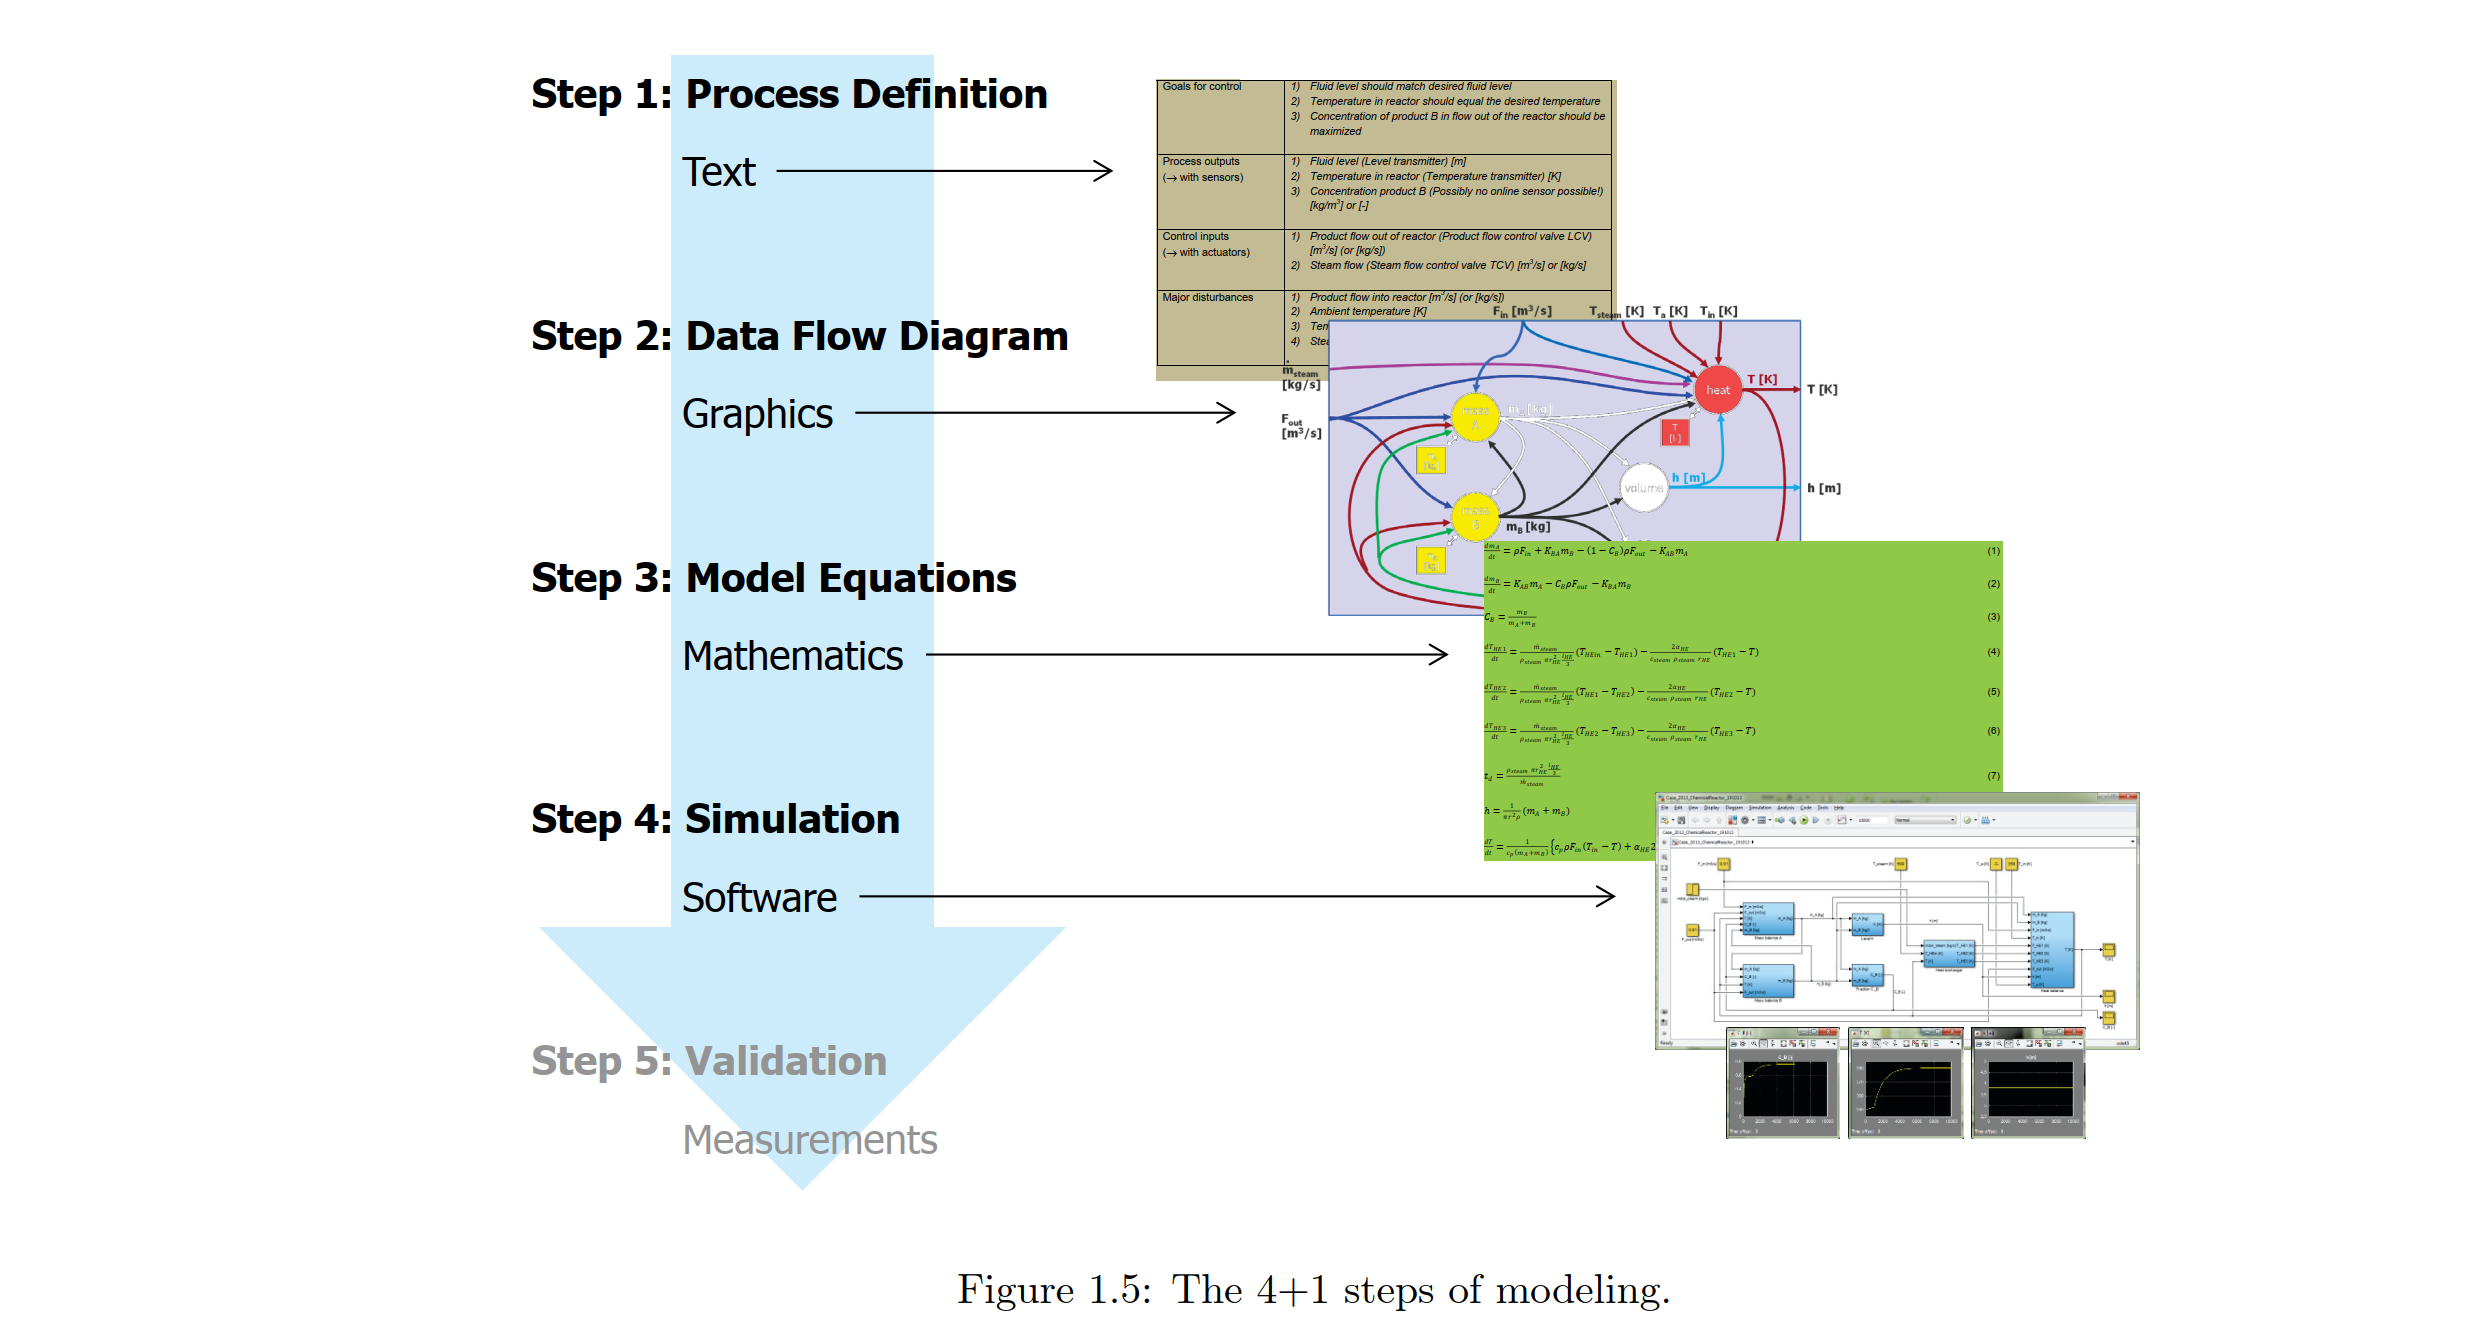
\includegraphics[
%	width=1\linewidth,
%	height=\paperheight,
%	keepaspectratio,
%	]{4+1Approach}
%	\caption{4+1 steps of modeling}
%	\label{fig:4+1}
%\end{figure}
%\pagestyle{empty}
%
%Starting from the process definition, model equations are derived with the help of a data flow diagram that lead to a simulation in software, e.g. Matlab. If possible, in the "+1" step, this model is validated with the real system.
%
%\section{Process Defintion}
%For object manipulation and other tasks, a robot arm needs to move to desired positions or track a given path. As the process focusses on the endpoint position of the robot arm, the process output can be defined as the xyz-position of the toolhead in space. The input, which can be used to control this output is the desired position. Another input that effects the output are objects attached to or carried by the robot arm. These can be considered disturbance inputs. From this, the process definition can be derived as seen in \ref{tab:ProcessDefinition}.
%
%\begin{table}[H]
%	\centering
%	\caption{Process Definiton}
%	\begin{tabular}{ll}
%		Goal for control:& Endpoint position of Robot arm   \\
%		Process output: & Endposition of Robot arm
%		 (sensor: measured with pulse encoders on the axes)   \\
%		Control inputs: & Electric power to the actuators
%		 (actuator: motor)  \\
%		Major disturbance & Carried object  
%	\end{tabular}
%\label{tab:ProcessDefinition}
%\end{table}

	\renewcommand{\bibname}{References}
	\printbibliography
	\newpage
	
	
	\begin{appendices}
		\chapter{Appendix 1}
		\chapter{Appendix 2}
	\end{appendices}
	
	
	
\end{document}

%Questions for Report writing:Ton.ammerlaan@han.nl
